% -*- mode:LaTeX; mode:visual-line; mode:flyspell; fill-column:75 -*-

\documentclass[conference]{IEEEtran}

% numbers option provides compact numerical references in the text.
\usepackage[numbers,sort]{natbib}
\usepackage{multicol}
\usepackage[bookmarks=true]{hyperref}
\usepackage{microtype}
\usepackage{todonotes}
\usepackage{mathtools}
\usepackage{amsfonts}
\usepackage{cleveref}

% -*- mode:LaTeX; mode:visual-line; mode:flyspell; fill-column:75 -*-

\newcommand*{\parens}[1]{\left( #1 \right)}
\newcommand*{\paren}[1]{\left( #1 \right)}
\newcommand*{\braces}[1]{\{ #1 \} }
\newcommand*{\brackets}[1]{\left[ #1 \right] }

\newcommand{\argmin}[1]{\ensuremath{\underset{#1}{\arg \! \min}\;}}
\newcommand{\argmax}[1]{\ensuremath{\underset{#1}{\arg \! \max}\;}}


\pdfinfo{
   /Author (Homer Simpson)
   /Title  (Robots: Our new overlords)
   /CreationDate (D:20101201120000)
   /Subject (Robots)
   /Keywords (Robots;Overlords)
}

\begin{document}

\title{Inferring Controllers from Natural Language Instructions}

% You will get a Paper-ID when submitting a pdf file to the conference system

\newcommand{\authorSpace}{\hspace{20pt}}
\author{
\authorblockN{
Felix Duvallet \authorSpace
Klas Kronander \authorSpace
Aude Billard}
\authorblockA{
  Learning Algorithms and Systems Laboratory\\
  \'{E}cole Polytechnique F\'{e}d\'{e}rale de Lausanne\\
  \texttt{\{felix.duvallet, klas.kronander, aude.billard\}@epfl.ch}
}
}


\maketitle

\IEEEpeerreviewmaketitle

% -*- mode:LaTeX; mode:visual-line; mode:flyspell; fill-column:75 -*-
\section{Introduction}
\label{secIntroduction}

Enabling robots to understand natural language would provide an intuitive interface between lay users and complex robots.
Prior work on enabling robots to understand language has addressed diverse tasks such as following route directions through indoor and outdoor environments~\cite{macmahon06, kollar10, matuszek12a, duvallet13, boularias15}, mobile manipulation~\cite{tellex11, howard14a}, or building semantically-annotated maps of the environment~\cite{walter13}.
These approaches typically map language to robot plans or high-level symbolic robot languages, and assume a controller exists that can adequately execute the desired actions.
Hence, natural language has been used mainly as a means of communicating final or intermediate task goals to the robot (e.g., route directions), but not in specifying \emph{how} to reach those goals.
Our work addresses this gap by leveraging the expressiveness of language and the power of Dynamical Systems-based motion generation.
This could enable language-based control of robots performing complex tasks that require reasoning at the trajectory level.

Dynamical Systems (DS) based approaches have emerged as an extremely effective means of generating robot trajectories, and provides several key benefits over planning-based approaches:
they are robust to perturbations of the robot,
they are robust to perturbations in the environment,
and they generalize well across entire families of trajectories.
Such DS models are usually tailored to specific tasks via learning from demonstration or reinforcement learning for tasks such as reaching a target point~\cite{KhansariZadeh2011,Calinon2012} or repeating a pattern~\cite{Buchli2006}.
Connecting natural language and Dynamical Systems would enable users to communication both \emph{what} to do and \emph{how} to do it in a unified representation.

In this report, we explore natural language for online modification of DS models belonging to a recent framework allowing incremental learning in stable DS models proposed by \citet{Kronander2015}.
We train a model from human demonstrations of the desired behavior modifications (using kinesthetic teaching), and generalize those to novel environments.
During execution, the user can then change the behavior of robot (through the controller) by using the trained natural language commands instead of requiring more manual interaction.
This ability can be especially advantageous when the user is unable to interact physically with the robot, either due to safety constraints or a disability.

\begin{figure}[t]
  \centering
  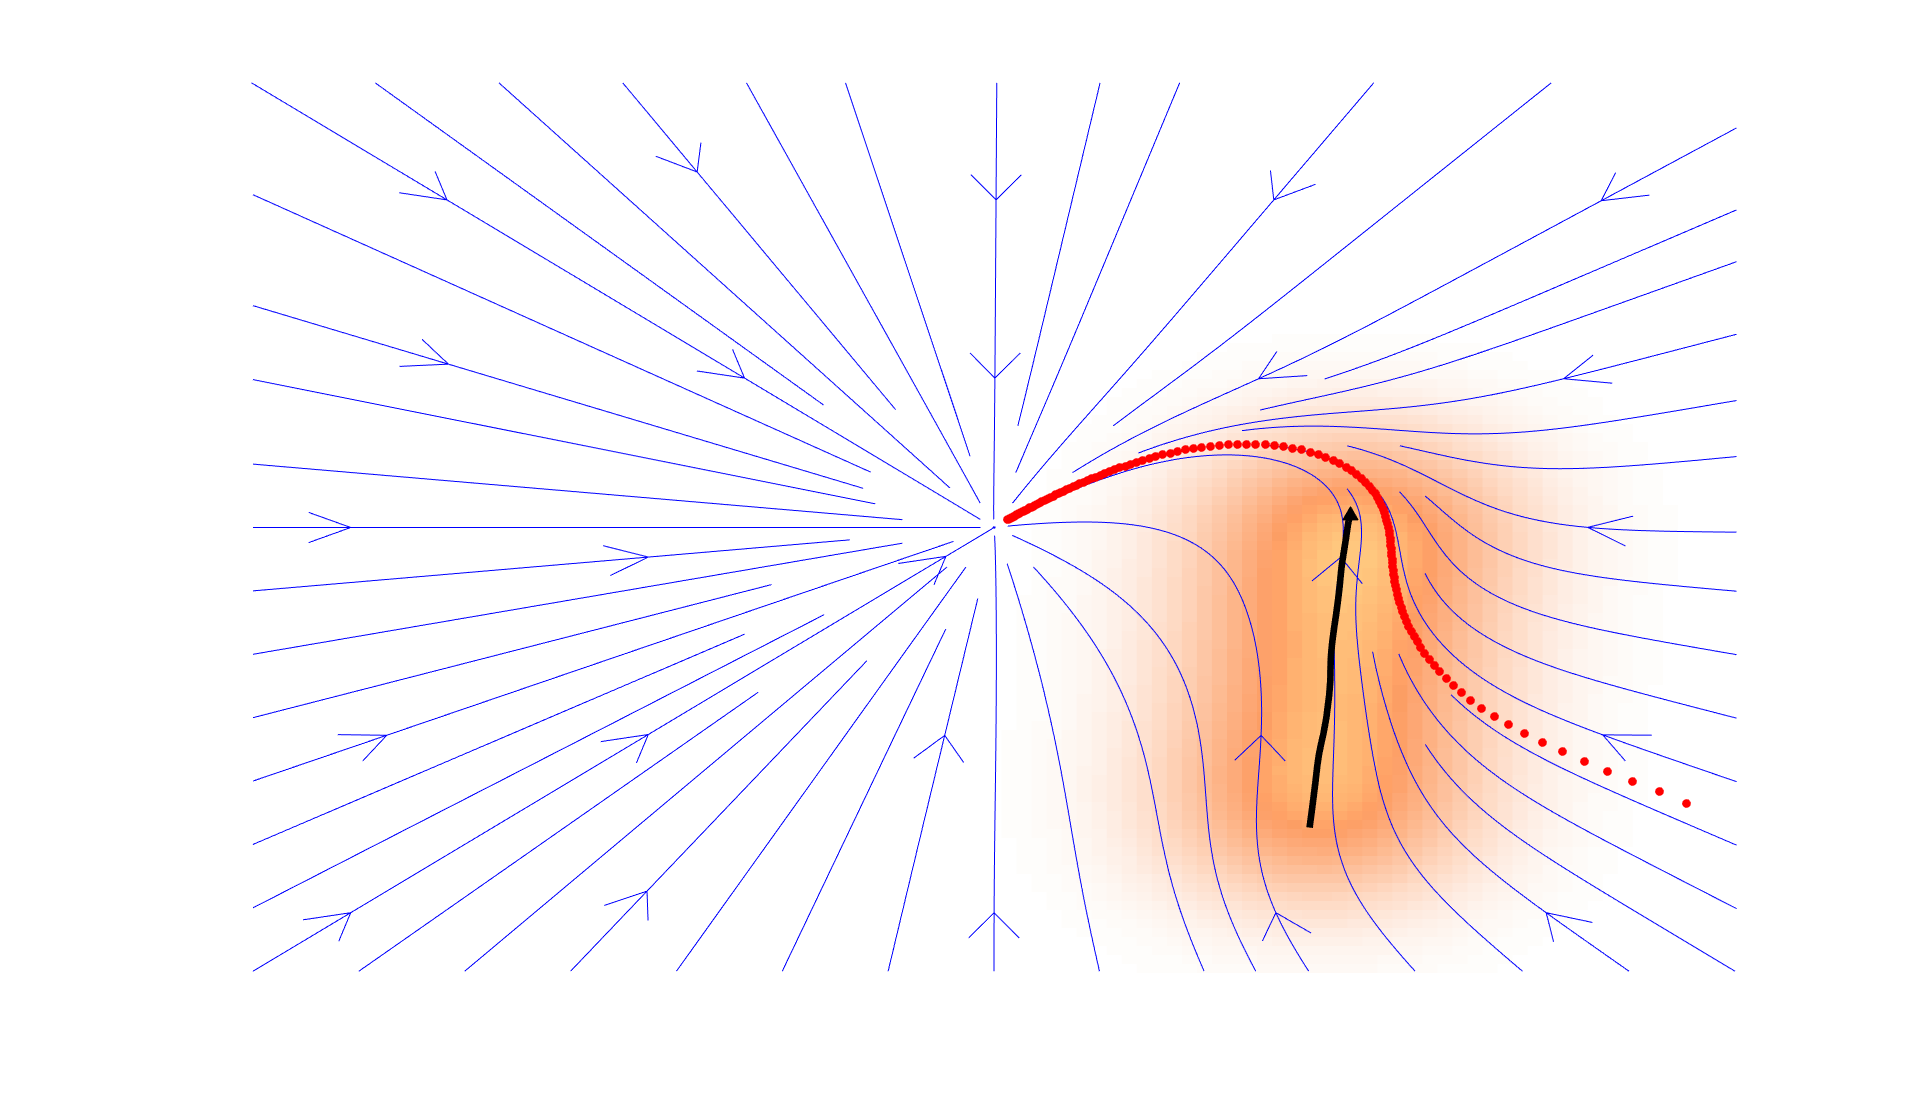
\includegraphics[
    % trim = left bottom right top
    trim = 150mm 50mm 100mm 80mm, clip,
    width = 0.4\textwidth,
  ]{figs/gp_figs/3a-traj1.png}
  \caption{A Modified Dynamical System, representing the controller policy over the entire state space (a 2D plane in this example): at every point the robot follows the gradient until it reaches the attractor.
 In the colored areas, the user has provided a correction to the policy (black arrow), which updates the policy in the same region of state space (re-shaped blue lines),
 resulting in behavior that generalizes to other nearby areas of the state space: for example the red trajectory.
    Our goal is to use natural language to modify a dynamical system, resulting in trajectories that performs the desired behavior.
}
  \label{figProblemSetup}
\end{figure}



% For example, an assistive robot may need to understand how much pressure it should exert when cleaning a patient's skin,
% or a factory robot may need to change how stiffly it should hold a part when cooperatively holding it for a person to assemble,
% or a <> robot may need to know from which direction to approach an object


% -*- mode:LaTeX; mode:visual-line; mode:flyspell; fill-column:75 -*-


\section{Approach}
\label{sec:approach}

\subsection{Modified Dynamical System}
In this work, we model the desired motion of the robot with a first order autonmous DS:
\begin{equation}
  \label{eq:DS_general}
  \dot x = f(x)
\end{equation}
where $x \in \mathbb{R}^3$ is the position of the end-effector of the robot with respect to an external coordinate frame. We will exclusively consider DS models that are stable at a single attractor point. Specifically, we use Locally Modulated Dynamical Systems (LMDS), which uses a basic DS model with known stability properties $\dot x = f^o(x)$ and achieves flexibility by reshaping this model locally:
\begin{equation}
  \label{eq:DS_reshaped}
  \dot x = f(x) = M(x)f^o(x)
\end{equation}
where $M(x)$ is a matrix valued function that rotates and scales the original dynamics in a continous manner accross the workspace. An example is given in Fig. \ref{figProblemSetup}, which plots the integral curves of a DS over 2d space. In this case, the original dynamics is a linear system and the DS is locally rotated in the right part of workspace. The procedure of reshaping the DS such that it locally aligns with incrementally arricing training data is described in detail in \todo{add reference to klas's RAS paper}.
\subsection{Demonstrations}

\subsection{Inferring Controllers from Language}

We begin with a Dynamical System (DS) that encodes the robot goal using an attractor point.
The attractor is simply the state the robot is attempting to reach, and the DS dynamics specify how the

Once the user specifies a natural language command, we infer a Modified Dynamical System (MDS) using the learned corrections described previously.


\todo[inline]{Describe a MDS, how it's different from a DS, and how to learn the modifications}


% -*- mode:LaTeX; mode:visual-line; mode:flyspell; fill-column:75 -*-
\section{Experiments and Results}
\label{sec:results}

We now present proof-of-concept experiments on a robot reaching task.
These early results serve as an initial demonstration of our ability to learn the correct behavior from user demonstrations and apply those when the user provides natural language command during task execution.

The robot is tasked with reaching a goal, and the initial Dynamical System is a linear dynamics model with a stable attractor at the goal position; this results in straight-line trajectories towards the goal.
While this initial behavior correctly specifies the task (the \emph{what}), changes in the environment (such as the addition of a bin) may result in the robot incorrectly performing the task, as shown in \Cref{figExperimentSetup}.
Note that in our experiments the robot has no sensors to detect obstacles.
The training phase consisted of a single demonstration with the user back-driving the robot under the original dynamics with the utterance ``go up''.

During the experiment, the user (though natural language) helps the robot to complete the task correctly by reshaping the Dynamical System using the learned correction (invoked using the same utterance).
In this work we used text-based input with no delay, using a speech-to-text engine would be straightforward but would introduce additional delays, handling those remains future work.
In this scenario the robot is able to complete the task without hitting the box, and can generalize to different starting positions.
Additionally, using the same learned correction the user could modify the dynamics on a different task (reaching inside a box in another location).

\begin{figure}[t]
  \centering
  \begin{tikzpicture}
    \draw (0, 0)
    node[name=image, anchor=south west, inner sep=0pt, outer sep=0pt]{
      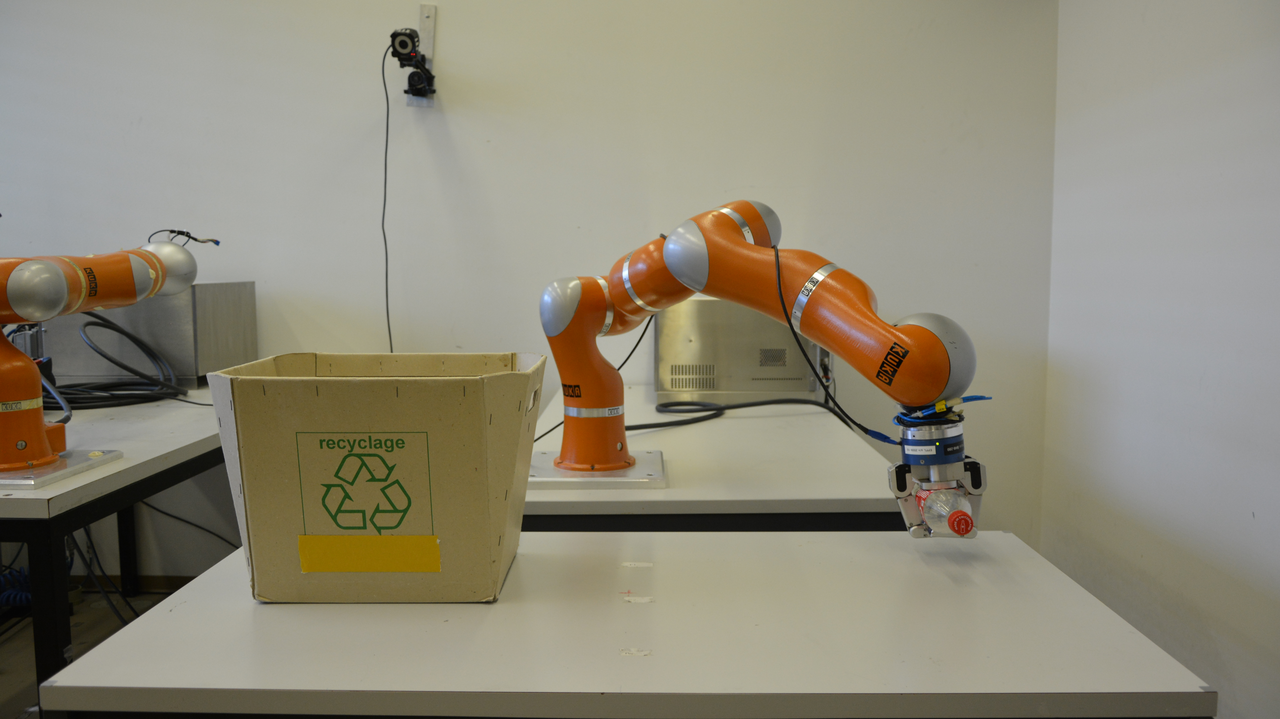
\includegraphics[
        % trim = left bottom right top
        trim = 18mm 5mm 20mm 15mm, clip,
        width = 0.4\textwidth
      ]{figs/setup-start.png}
    };
    \begin{scope}[x={(image.south east)},y={(image.north west)}]

      %% Grid
      %% \draw[help lines,xstep=.1,ystep=.1] (0,0) grid (1,1);
      %% \foreach \x in {0,1,...,9} { \node [anchor=north] at (\x/10,0) {0.\x}; }
      %% \foreach \y in {0,1,...,9} { \node [anchor=east] at (0,\y/10) {0.\y}; }

      \node[] (goal) at (0.2, 0.4) {};
      % List all the starting positions here (first is the actual hand).
      \foreach \x/\y in {0.85/0.3, 0/0, 0.6/0.1, 0.2/0.9, 0.4/0.9, 0.9/0.8} {
        \node[] (start) at (\x, \y){};
        \draw[->, blue, ultra thick, shorten >= 5pt] (start) -- (goal);
      }

    \end{scope}
  \end{tikzpicture}
  \caption{
    From the start position shown, the robot must place the bottle into the basket.
    However, the initial Dynamical System is unaware of the geometry of the basket, and the original trajectories are straight lines (shown in blue).
    Using the language description ``go up,'' the robot is able to infer a modification to the DS in order to execute the task correctly.
  }
  \label{figExperimentSetup}
\end{figure}


% -*- mode:LaTeX; mode:visual-line; mode:flyspell; fill-column:75 -*-
\section{Conclusions}
\label{secConclusions}



\clearpage

%% Use plainnat to work nicely with natbib.
\bibliographystyle{plainnat}
\bibliography{references}

\end{document}
